%Esta plantilla la usamos desde el 2018, si tienen alguna obervación pra mejorar, por favor mándenme un correo
% vvazquez@fcfm.buap.mx

\documentclass{siep}
\usepackage[spanish]{babel}
\usepackage[utf8]{inputenc}
\bibliographystyle{dcu}
\usepackage{cite}
\spanishdecimal{.}

\title[Una Revisi\'on de M\'etodos de Evaluaci\'on Econ\'omica en Saluds]{Una Revisi\'on de M\'etodos de Evaluaci\'on Econ\'omica en Salud}

\author[ad1][]{Joaqu\'in Viola-Chiazzaro}
\author[ad2][]{Ramon Alvarez-Vaz}




\correspondingauthor{Second AUTHOR} %aquí se determina al autor de correspondencia

\address[ad1]{Instituto de Estadística, Facultad de Ciencias Económicas y de Administración,\\ Universidad de la Rep\'ublica, Montevideo, Uruguay, Gonzalo Ramírez 1926, Piso 1 Of. 22 CP: 11200\\  e-mail: \url{joaquin.viola@fcea.edu.uy}\\ORCID \url{https://orcid.org/0009-0007-4385-9893}}
\address[ad2]{Instituto de Estadística, Facultad de Ciencias Económicas y de Administración,\\ Universidad de la Rep\'ublica, Montevideo, Uruguay, Gonzalo Ramírez 1926, Piso 1 Of. 20.1 CP: 11200\\  e-mail: \url{ramon.alvarez@fcea.edu.uy}\\ORCID \url{https://orcid.org/0000-0002-2505-4238}}
%\authors{First name LAST NAME \!$^{a}$, Second AUTHOR \!$^{a, b,}$\thanks{Corresponding author. \newline The authors are listed in}. \,\,,\\ Third AUTHOR \!$^{b}$}
%\addresses{$^{a}$\! Insti-ute of xxx xxx xxx xxx\\ University of xxx xxx, Address xxx xxx xx xxx xxx\\ e-mail: \url{xxx xx xxx}\\\medskip $^{b}$\! Second affiliation}

\Runauthors{Joaqu\'in Viola-Chiazzaro \it{et al.}} %Aquí puede ponerse el nombre del primer autor et al
%\Runauthors{J. Doe}
%\Runauthors{J. Doe and M. John}

%PLEASE DO NOT MODIFY OR REMOVE THESE!
%\Year{}
%\Vol{}
%\No{}
%\Startpage{}
%\Endpage{}
%\DOI{}
%\Received{}
%\Revised{}
%\Rerevised{}
%\Accepted{}
%\bibliographystyle{dcu}

\begin{document}
\begin{abstract}
En este trabajo se presenta una s\'intesis sobre distintos métodos de evaluación económica en la salud, mostrando el análisis costo-beneficio, costo-utilidad pero prestando especial interés en el análisis costo-efectividad.
A trav\'es de una breve introducción se muestran los distintos aspectos a tener en cuenta a la hora de hacer una evaluación económica, cómo la obtención de los datos sobre los costos de los tratamientos, así como de las medidas de efectividad y su obtención.
Se introduce el concepto del ratio incremental de costo-efectividad y el incremento del beneficio neto como herramientas para la toma de decisiones.
Se presentan métodos frecuencistas de intervalos de confianza y métodos de bootstrap para las estimaciones de los parámetros de costos y de efectividad, para la evaluación económica de tratamientos médicos.

\end{abstract}

\begin{keywords}
Evaluación Económica en Salud; Análisis Costo-Efectividad; Sistema Sanitario; Análisis Bayesiano; Inferencia Estadística
\end{keywords}
\maketitle

\section{Introducci\'on}
\label{sec:Intro}
La evaluación económica en el ámbito de la salud es un área que ha tenido un constante desarrollo en las últimas décadas. Cómo en la mayoría de los problemas económicos, la evaluación económica de tratamientos médicos busca determinar la distribución óptima de los recursos (que son limitados), en las distintas demandas (que pueden ser ilimitadas).

En este documento se trabaja con los casos en los que se desea evaluar dos tratamientos médicos, que en general tienen distintos costos, y distintos resultados.

En la primera parte se busca brindar una aproximación a los métodos de evaluación económica más usados, prestando principal interés en la evaluación de costo-efectividad. También en cómo obtener los resultados de costo y efectividad para aplicar las técnicas de evaluación, y en la interpretación de los resultados


\section{Evaluación Económica}
\label{sec:EE}

Los métodos de evaluación económica, surgen de resolver el problema económico de asignar recursos limitados, para maximizar los beneficios,  y conforman un conjunto de técnicas que pretenden medir los resultados de varias alternativas, y sirven de apoyo para la toma de decisiones. No buscan reducir los costos, si no guiar a los tomadores de decisiones en la mejor opción de gastar los recursos según los resultados obtenidos.
Usualmente se utilizan para comparar dos alternativas de inversión, por ejemplo en dos proyectos distintos, o para tomar la decisión de invertir en algo o no, cómo puede ser el arreglo de una máquina en una empresa de producción, o el cambio de una máquina por una más nueva.

\subsection{Evaluación Económica En Salud}
\label{sec:EES}
En el sistema sanitario en general, surge el problema de tener recursos limitados, para atender necesidades ilimitadas,  a lo que se suma que los tratamientos tienen costos altos, por lo que aparece la necesidad de aplicar métodos de evaluación económica para comparar dos tratamientos frente a una enfermedad, para tomar la decisión de seguir con el actual, o cambiar a un nuevo tratamiento (\cite{moreno_bayesian_nodate}). A su vez, \cite{weinstein_foundations_1977} plantean que la sociedad debe maximizar los beneficios agregados, lo que motiva la necesidad de aplicar una metodología que una los costos de los tratamientos, junto a los resultados de los mismos ( qué no están medidos en términos monetarios)

Desde la década del 1970, ha habido un aumento en la demanda de la atención médica, lo que ha generado un aumento en la cantidad de intervenciones disponibles,  y esto ha llevado a que los tomadores de decisiones para los gastos médicos necesiten estar más informado sobre los resultados y los costos para poder tomar mejores decisiones. Algunos de los factores principales que ha llevado a la necesidad de comparar costos y beneficios en el sistema sanitario son: el aumento de la población mayor, consecuencia de un aumento en la esperanza de vida, el aumento de la presencia de patologías crónicas y degenerativas, la mejora en las técnicas de diagnósticos, las innovaciones tecnológicas que generan mejores resultados en salud pero tienen mayores costos (\cite{baio_bayesian_nodate}) (\cite{soto_alvarez_evaluacion_2012}).

Existen agencias a nivel nacional e internacional que hacen estos análisis para poder brindar mayor información a quienes toman las decisiones a nivel gubernamental (\cite{zarate_evaluaciones_2010}). Por otro lado se observa, que a mayor progreso médico alcanzado, hay un mayor costo para obtener aún mejores resultados. (\cite{sacristan_evaluacion_nodate})


El desarrollo de esta área ha generado el interés de numerosos investigadores que han incursionado en las técnicas y las metodologías para la toma de decisiones. Esto ha generado un crecimiento exponencial de artículos sobre análisis económico en salud en las últimas décadas. Como por ejemplo ``Análisis de coste-utilidad de un programa de vigilancia para prevenir la luxación de cadera en niños y niñas con parálisis cerebral'' de \cite{vallejo-torres_cost-effectiveness_2021}, ``Once años de evaluaciones económicas de productos sanitarios en la Red de Agencias de Evaluación. Calidad metodológica e impacto del coste-utilidad'' de \cite{gimenez_once_2021}.\\


Nota: en el desarrollo del documento se hablará indistintamente de medicación, tratamiento y tecnología, salvo que se indique lo contrario.

\subsection{Distintos Métodos de An\'alisis}
\label{sec:DMA}
Existen distintos métodos para la comparación de tecnologías basados en los resultados y los costos de las mismas.Por lo general se busca comparar tratamientos alternativos, contra el tratamiento actual, o status quo, en algunos casos más avanzados se comparar\'an más de dos alternativas.Estos métodos se diferencian principalmente en la forma de medir los resultados, y nosotros los separaremos en los 3 principales: costos-beneficios, costos-utilidad y costo-efectividad. Este último será el que nos resultará de principal interés.

\subsubsection{Análisis Costos-Beneficios}
\label{sec:ACB}
Para el análisis costos-beneficios es necesario tener los costos y efectos medidos en la misma escala, usualmente en términos monetarios.
En estos casos el criterio de selección es que $Beneficio > Costo$, y en particular se maximiza $Beneficio-Costo$. Surge inmediatamente la relación de este análisis con la teoría económica del bienestar, dónde el bienestar social es la suma de los bienestares individuales. Por ese motivo hay lograr expresar todos los costos, beneficios y prejuicios para la salud en términos monetarios (\cite{baio_bayesian_nodate}),con la ventaja de poder medir tratamientos que tienen distinta medida de efectividad, pero la dificultad de transformar las ``unidades de salud'' en unidades monetarias.

El Análisis Costo-Beneficio comunmente se lo relaciona con la teoría estandar económica del ''Bienestar Social'', donde el Bienestar Social se calcula como la suma de los bienestares individuales (\cite{gray_applied_2011}). El presupuesto debe ser asignado de forma tal que se maximice el bienestar social.\

Para la realización del Análisis Costo-Beneficio es necesario tener los resultados de los tratamientos medidos en unidades monetarias, el principal problema radica en obtener una estimación del valor monetario del beneficio social alcanzado por cada una de los tratamientos (\cite{soto_alvarez_evaluacion_2012}).\

Una de las principales ventajas de aplicar este método es que se puede comparar dos tratamientos en los que sus resultados miden variables distintas, es decir, su efectividad está medida en distintas medidas. Por ejemplo, si debemos destinar un presupuesto limitado en tratamientos para distintas enfermedades, como un tratamiento para el cáncer de mama y otro contra el VIH, si logramos expresar los resultados en términos monetarios para el bienestar social podremos hacer un análisis costo-beneficio.\\
La necesidad de expresar en términos monetarios los resultados de un tratamiento ha llevado a que esta técnica no sea muy aplicada.



Estos análisis buscan estimar el monto que los pacientes estarían dispuestos a pagar por mejorar su estado de salud, (mitigar dolores, reducir el estres) o el valor con el que habría de compensarolos por empeorar su estado de salud.\
Inicialmente se utilizaban los costos que suponían la pérdida de productividad por la enfermedad, y no se consideraba la salud en si misma y los costos asociados a actividades no remuneradas. Por lo que este análisis mostraba muchas deficiencias.

\subsubsection{Valoración Económica de los resultados}
\label{sec:VER}
Uno de los métodos utilizados son los ''Métodos de Preferencias Económicas'', que utilizan encuestas sobre el comportamiento y los intereses frente a distintas situaciones hipotéticas para poder estimar la disposición a pagar de los individuos para mejorar su estado de salud frente a distintas situaciones, o el valor por el que espera se compensado por no recibir los beneficios del tratamiento.
La encuesta debe constar con información socio-económica del entrevistado para poder validar los resultados, también se deben presentar los resultados previstos para el tratamiento y los posibles efectos adversos.\\
Un problema de esta metodología es que se están presentando situacions hipotéticas, y puede generar sesgos en las respuestas. Como el sesgo hipotético y el estratégico, el primero refiere a la clara diferencia entre una situación hipotética y una real, ya que en caso de necesitar efectivamente un tratamiento podría estar dispuesto a pagar más del que se creía. El segundo tipo de sesgo refiere a la creencia de que podría llegar a necesitar de ese tratamiento, y si responde un valor bajo podría influir sobre el costo final, y así pagar menos de lo que estaría dispuesto en caso de necesitarlo efectivamente (\cite{soto_alvarez_evaluacion_2012}).\\
Otro problema son los asuntos éticos, y la incomodidad de los encuestados a responder en cuanto a la valorización que hacen a aspectos cómo la discapacidad o el derecho a acceder a la salud.

Otra opción, bastante más simple, es conocer los costos asociados a la prevalencia de determinada enfermedad, y las probabilidades de contraerla. Para esto siguiendo el ejemplo del libro \textit{Bayesian Methods In Health Economics, de Gianluca Baio} (\cite{baio_bayesian_nodate}), que plantea la administración de una vacuna para niños, (hipoteticamente 100\% efectiva), y los dos tratamientos posibles es aplicarlo solo a los niños de la escuela, o también a los liceales. Se asume en caso de contraer la enfermedad, se deberá tener una semana de hospitalización a costo $h$.\

Se presenta la siguiente tabla \ref{tabla:2} con el tamaño de la población escolar $N_1$ y liceal $N_2$ y las probabidades de contraer la enfermadad $\rho_1$ y $\rho_2$ para  cada población. El costo de administración de cada vacuna $v$ es $\$12$, y el costo de hospitalización $h$ por una semana es $\$700$

\begin{table}[htbp]
	\centering
	\begin{tabular}{lcc}
		\hline
		& Escolares (1) & Liceales (2) \\ 
		\hline
		Tamaño población (N) & 4.093.710 & 3.252.140 \\ 
		Probabilidad de enfermar ($\rho$) & 0.1427 & 0.0548 \\ 
		\hline
	\end{tabular}
	\caption{Ejemplo 2}
	\label{tabla:2}
\end{table}

Entonces, el tratamiento 1, que es aplicarle la vacuna solo a los niños en edades escolares tiene un costo $c_1 = v\times N_1=\$49124520$, y el costo del tratamiento 2, que es aplicarle la vacuna a ambas poblaciones sería $c_2 = v\times(N_1+_N2)=\$88150200$

Luego, la parte de los beneficios se puede ver como el ahorro que supone tener a la población inmunizada, en el sentido de que no se tendrá el costo de hospitalización porque no habrá población que contraiga la enfermedad.\\
El beneficio de aplicar el tratamiento 1 será $b_1=h\times N_1\times \rho_1=\$408920692$ y el beneficio del tratamiento 2 es $b_2=h \times(N_1\times\rho_1 + N_2\times\rho_2)=\$533672790$.

Luego, el beneficio neto de cada tratamiento se calcula como la resta de los beneficios menos los costos, $BN_1=b_1-c_1=\$359796172$ y $BN_2=b_2-c_2=\$445522590$, por lo que el tratamiento 2, de vacunar a los estudiantes de escuela y liceo es el que produce el mayor Beneficio Neto.

\subsubsection{Análisis Costos-Utilidad}
\label{sec:ACU}
Se usa para casos especiales del análisis costos-efectividad, particularmente cuando la efectividad está medida en \textit{QALY's} (Quality-Adjusted Life Years), años de vida ajustados por la calidad.
\textit{QALY} es una medida compuesta de los efectos, integrada por las dos dimensiones principales de la salud, la cantidad y la calidad. Puede interpretarse como años de vida saludables equivalentes al estado de salud real.

El Análisis de Costo-Utilidad se suele ver como un caso puntual del Análisis de Costo-Efectividad, en donde comparamos dos tratamientos según los años de vida ganados, ajustados por la calidad, lo que en la sección 2.3 se presentó cómo \textbf{QALY (Quality-adjusted life years)}, que son los años de vida ganados, multiplicados por \textbf{HRQL (Health-related quality life)}.\\
Una de las principales ventajas de la utilización del \textbf{QALY} es que se la da importancia a la calidad de vida de los pacientes, obteniendo iguales resultados un paciente que gana 10 años de vida con una calidad de 0.5 que un paciente que gana 5 años de vida, con una calidad de 1 (óptima), comparar los valores de HRQL para cada tratamiento nos permite poder comparar los tratamientos en términos de ''salud''.

\

En este caso, la ''utilidad'' hace referencia a la preferencia de los pacientes por un estado de salud u otro, o a la calidad de vida recibida.
La utilidad se ve reflejada por valores entre 0 y 1, donde 0 representa el peor estado de salud posible, y 1 el óptimo, estos valores pueden ser calculados aplicando los cuestionarios presentados anteriormente.

\

Para el tratamiento $t$ podemos calcular la calidad de vida $q$ en el momento $j$ ($q_{tj}$), como el promedio de la utilidad entre el momento j, y el momento j-1, por la fracción de años que hay entre j-1 y j.

\begin{equation}
q_{tj} = \frac{u_{t(j-1)}+u_{tj}}{2}\delta_j
\end{equation}

Donde $\delta_j$ = tiempo entre j-1 y j, medido en años.

\

En \textit{''Bayesian Methods in Health Economics de Gianluca Baio''} (\cite{baio_bayesian_nodate}) tenemos un ejemplo donde se calcula la calidad de vida cada 6 meses durante dos años para dos pacientes, uno de cada tratamiento, teniendo los tiempos j=1,2,3,4, y luego, $e_t=\sum_{j=1}^4 q_{tj}$ es la efectividad para cada tratamiento.

\begin{table}[ht]
	\centering
	\begin{tabular}{lcccccr}
		\hline
		& Inicio & 6 meses & 12 meses & 18 meses & 24 meses & Total \\ 
		\hline
		\textbf{Tratamiento 1} \\
		Utilidad & 0.656 & 0.744 & 0.85 & 0.744 & 0.744 & \\ 
		QALY's &  & 0.350 & 0.399 & 0.399 & 0.372 & 1,519 \\
		Costos &  & \$2.300 & \$300 & \$300 & \$ 300 & \$3.200 \\
		\hline
		\textbf{Tratamiento 0} \\
		Utilidad & 0.656 & 0.656 & 0.656 & 0.656 & 0.744 & \\ 
		QALY's &  & 0.328 & 0.328 & 0.328 & 0.350 & 1,334 \\
		Costos &  & \$300 & \$300 & \$300 & \$ 300 & \$1.200 \\
		\hline
	\end{tabular}
	\caption{Ejemplo 3 del libro Bayesian Methods in Health Economics}
	\label{tabla:3}
\end{table}

En el ejemplo vemos que se aplica la fórmula obtenida en (12) para calcular las QALY's en cada tramo de tiempo, por ejemplo $q_{11}=(0.656 + 0.656)/2 \times 0.5$, y por último obtenemos 1,519 de QALY's extra para el paciente del tratamiento 1 durante los dos años, y de 1.334 para el paciente del tratamiento 0, al costo de \$3.200 y \$1200 respectivamente.\\
Luego, con la diferencia de QALY's promedio, calculada con el resto de los paciente obtenemos la diferencia de efectividad, y lo mismo para los costos. Para así poder calcular el $ICER_{1,2}$ cómo ya se mostró anteriormente

\subsubsection{Análisis Costo-Efectividad}
\label{sec:ACE}
En esta técnica se comparan los tratamientos en términos de efectividad, como puede ser los años de \emph{vida ganados}, mejoras en el estado de salud, presión sanguínea o nivel de colesterol (sobre estas formas de medir la efectividad se profundizará en la siguiente sección).
En este caso, el costo y la efectividad no estan medidos en las mismas unidades, por lo que los criterios de selección pasan a ser un poco ambiguos. Para estos casos se debe fijar un monto fijo, de disposición a pagar (\emph{willingness to pay}) para aumentar la efectividad en una unidad. La eficacia es una medida de si un tratamiento cumple sus objetivos o no, la efectividad, involucra además la optimización de los recursos, mientras que la eficiencia es un concepto económico que relaciona estos dos términos.Como se comentó anteriormente, la evaluación económica mediante el análisis de costo efectividad busca comparar simultáneamente los costos (medidos en términos económicos) y la efectividad de los tratamientos (medidos justamente, en términos de efectividad). Para eso se considera  el  \textit{Ratio Incremental de Costo-Efectividad}, (\textbf{ICER}) por sus siglas en inglés, que medirá la variación de los costos según la variación en la efectividad.


La \textbf{efectividad} es la medida en la cual un tratamiento cumple con los objetivos para los que fue diseñado bajo circunstancias óptimas, teniendo medidas de resultados finales (por ejemplo años de vida ganados) y otras de resultados parciales (la carga viral o presión arterial) dependiendo del objetivo principal del tratamiento.
Muchas veces se utiliza cómo unidad de medida los años de vida ganados, o el aumento de la esperanza de vida ¿Pero qué pasa con la calidad de los años de vida? El \textbf{QALY's} es una medida de la efectividad que  pretende combinar los años de vida ganados y la calidad de estos años ganado según la intervención. Esto debido a que algunos tratamientos, si bien cumplen con su objetivo, pueden ser invasivos y dañar la salud en otros aspectos.

Para construir las \textit{QALY's} es necesario poder medir la calidad de vida, medida en \textbf{HRQL} (Health-related quality of life), cómo la calidad de los años ganados, asociado a cada intervención. 

Existen distintos instrumentos que buscan agregar el efecto de la calidad de los años de vida ganados,cuestionarios que suelen incluir variables como el dolor, la autonomía, estado de ánimo, morbilidad y preguntas sobre las actividades usuales, por ejemplo el \textit{EuroQol 5D (EQ-5D)} (\cite{baio_bayesian_nodate}) o el \textit{SF-6D }.


En general se usan ensayos clínicos  para asignar aleatoriamente  a los pacientes  uno de los tratamientos para minimizar el sesgo de los resultados. Se identifican todos los costos que se hacen durante  el estudio ( por ejemplo, ensayo clínico), y todos los recursos que son utilizados, expresados en términos monetarios, que se pueden  clasificar en  

\begin{itemize}
	\item \textbf{Costos Directos}: incluye todos los bienes y servicios usados durante el ensayo, el tiempo de los profesionales, los costos de los tratamientos.
	
	\item \textbf{Costos Indirectos}: También conocidos como costos de productividad, ya que están relacionados con los costos que tienen los pacientes por participar del ensayo clínico, cómo faltar al trabajo.
	
	\item \textbf{Costos Intangibles}: relacionados al dolor o sufrimiento que tienen los pacientes durante el ensayo.
	
	\item \textbf{Costos de Transición}: relacionado a los gastos de la investigación para la producción de nuevos tratamientos.
\end{itemize}

\subsubsection{Ratio Incremental de Costo-Efectividad}
\label{sec:RCICE}
Como se mencionó anteriormente, el Ratio Incremental de Costo-Efectividad (de ahora en adelante \textit{ICER}) es una herramienta que sirve para medir el incremento de los costos según el incremento en la efectividad al comparar 2 tratamientos. Así que al comparar el tratamiento 1, supongamos tratamiento alternativo, contra el tratamiento 0, tratamiento de control, estaremos calculando $ICER_{1,0}$.

Sea $\gamma_i$ y $\epsilon_i$ el costo y la efectividad asociados al tratamiento $i$, podemos ver el incremento del costo cómo $\Delta\gamma_{1,0}=\gamma_1-\gamma_0$ y el incremento de la efectividad $\Delta\epsilon=\epsilon_1-\epsilon_0$. Definimos el Ratio Incremental de Costo-Efectividad en la ecuación \ref{eq:ICER}:

\begin{equation}
ICER_{1,0}= \frac{\Delta\gamma}{\Delta\epsilon}
\label{eq:ICER}
\end{equation}

El $ICER_{1,0}$ es el aumento del costo por aumentar en una unidad la efectividad. A estar trabajando con muestras se debe estimar   $\widehat{ICER_{1,0}}$,  para lo que usan los costos y la efectividad promedio ($\bar{c}$ y $\bar{e}$) de cada uno de los tratamientos, por lo cual queda

\begin{equation}
\widehat{ICER_{1,0}}= \frac{\bar{c_1}-\bar{c_0}}{\bar{e_1}-\bar{e_0}}
\end{equation}

Hay observar que el valor del $\widehat{ICER_{1,0}}$ puede ser positivo o negativo según distintos factores, por lo que no se puede tomar cómo referencia un solo valor para decidir sobre los tratamientos

\begin{equation}
\widehat{ICER_{1,2}}
\begin{cases}
<0 & \bar{c_1} > \bar{c_2} \text{   y   }   \bar{e_1} < \bar{e_2} \\
<0 & \bar{c_1} < \bar{c_2} \text{   y   }   \bar{e_1} > \bar{e_2} \\
>0 & \bar{c_1} > \bar{c_2} \text{   y   }   \bar{e_1} > \bar{e_2} \\
>0 & \bar{c_1} < \bar{c_2} \text{   y   }   \bar{e_1} < \bar{e_2} \\
\end{cases}
\end{equation}

El valor del ratio incremental puede ser negativo ó positivo según distintos factores. Por ejemplo, si los costos promedios del tratamiento $0$ son más bajos que los del tratamiento $1$, y la efectividad del tratamiento $0$ es mayor que la efectividad del tratamiento $1$, el $\widehat{ICER_{1,0}}$ será negativo, pero si los costos del tratamiento $0$ son más altos que del tratamiento $1$, y la efectividad del tratamiento $1$ es mayor que la del tratamiento $0$ también se tendr\'a un valor negativo de $\widehat{ICER_{1,0}}$, y es evidente que en estas dos situaciones se deben tomar medidas opuestas, pero ambas tienen igual signo.Para eso el valor del $ICER_{1,0}$ se acompañas de una representación gráfica llamada ``Plano Costo-Efectividad" que aparece  en el gráfico \ref{fig:1}.
\
En el eje horizontal de nuestro plano encontraremos $\Delta\epsilon$, el incremento de la efectividad, y en el eje vertical tendremos $\Delta\gamma$, el incremento de los costos. Además, veremos que el plano está dividido en dos partes por una recta que pasa por el origen y tiene pendiente positiva \textbf{R}, esta recta nos divide el plano en las situaciones en las que elegiremos el tratamiento $0$ y en las que elegiremos el tratamiento $1$. Este valor de \textbf{R} representa la disponibilidad a pagar por una unidad extra de efectividad.

En nuestro plano, la zona coloreada en celeste, nos marca las situaciones en dónde elegiremos el tratamiento alternativo frente al tratamiento de control.
\
Se nota que en el cuadrante 4 (abajo a la derecha ó al Sur-Este), sube la efectividad y baja el costo, por lo que el resultado es inmediato. Mientras que en los cuadrantes 1 y 3 (arriba a la derecha y abajo a la izquierda respectivamente), debemos estar por debajo de la línea con pendiente \textbf{R}. Para el cuadrante 1, esto se cumple cuando $ICER_{1,0}<R$ mientras que en el cuadrante 3 cuando $ICER_{1,0}>R$. Por último, en el cuadrante 2 nunca optaremos por el tratamiento alternativo debido a que aumentan los costos y baja la efectividad.\

Además, cuando estamos en el cuadrante 4, en donde el tratamiento $1$ (alternativo) tiene mayor efectividad y menor costo que el tratamiento $0$, podemos decir que el tratamiento $0$ es \textbf{dominado} por el tratamiento $1$. Mientras que en el cuadrante 2, en dónde el tratamiento $0$ tiene mejores resultados en costo y efectividad que el tratamiento $1$, este último es \textbf{dominado} por el tratamiento $0$.

\begin{figure}[htbp]
	\centering
	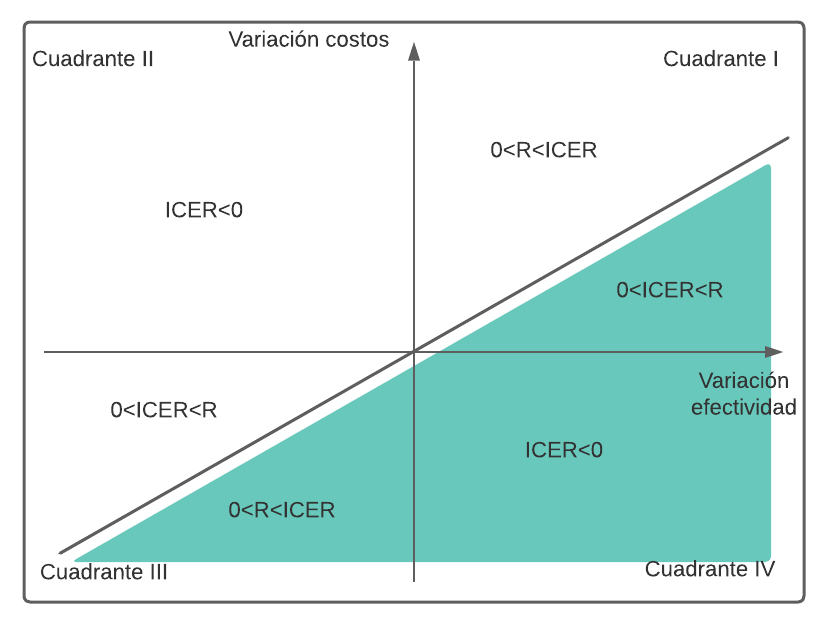
\includegraphics[width=0.45\textwidth]{grafi/Plano_Costo_elab_propia.png}
	\caption{Plano Costo-Efectividad \textit{elaboración propia}}
	\label{fig:1}
\end{figure}

\subsubsection{Incremento del Beneficio Neto}
\label{sec:IBN}
El Incremento del Beneficio Neto (\textit{INB}) busca mejorar el \textit{ICER} en el sentido de que es más fácil de interpretar, con valores positivos ya podemos tomar una decisión. Pero para esto es necesario haber fijado el valor de \textbf{R} previamente.

\begin{equation}
INB_{1,0} = R(\epsilon_1-\epsilon_0)-(\gamma_1-\gamma_0) = R\Delta\epsilon-\Delta\gamma
\end{equation}

El \textit{INB}  está expresado en términos monetarios, dado que que los costos lo están, \textbf{R} también lo está, y multiplica la efectividad que no tiene ninguna unidad de medida particular. Si la diferencia en la efectividad de un tratamiento a otro, multiplicada por la voluntad a pagar por cada unidad de efectividad extra, supera la diferencia de los costos, se cambiará de tratamiento.Para obtener tener la estimación de \textit{INB} se usan los costos y la efectividad promedio.

\begin{equation}
\widehat{INB_{1,0}} = R(\bar{e_{1}}-\bar{e_{0}})-(\bar{c_{1}}-\bar{c_{0}})
\end{equation}

El $\widehat{INB}$ es una combinación lineal de parámetros que se puede estimar,  para lo cual se puede calcular la esperanza y la varianza. 

\begin{equation}
\mathbb{E}(\widehat{INB_{1,0}})=R(\epsilon_1-\epsilon_0)-(\gamma_1-\gamma_0)
\end{equation}

\begin{equation}
\mathbb{V}(\widehat{INB_{1,0}})=\sum_{i=0}^1(R^2\sigma^2_{e_i}+\sigma^2_{c_i}-2R\rho_i\sigma_{c_i}\sigma_{e_i})/n_i
\end{equation}

En donde la $\mathbb{V}(\widehat{INB})$ se puede estimar con el estimador de la varianza ($\widehat{\mathbb{V}(\widehat{INB})}$) sustituyendo los desvíos ($\sigma$) por los desvíos muestrales $s$, y la correlación ($\rho$) por la correlación muestral $r$.

Se puede luego construir la curva de aceptación de costo-efectividad, donde  la misma mide la probabilidad de que $INB_{1,0}$ sea positivo para distintos valores de R, esto es $P(\widehat{INB_{1,0}}>0)$. Para valores de R bajos, cuando la disposición a pagar por una unidad más de efectividad es baja, la probabilidad de que $\widehat{INB_{1,0}}$ sea positivo es muy baja, y para valores altos de R, tiende a 1.

\begin{figure}[htbp]
	\centering
	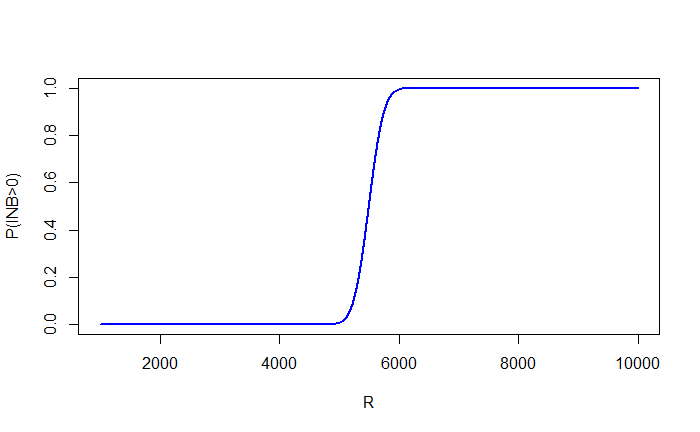
\includegraphics[width=0.45\textwidth]{grafi/Curva_acept.jpg}
	\caption{Curva de Aceptación}
	\label{fig:2}
\end{figure}

\subsection{Determinación del valor de ``R''}
\label{sec:DVR}

Una de las interrogantes que nos queda al momento es cómo determinamos el valor máximo que estamos dispuesto a pagar por una unidad extra de efectividad, lo que anteriormente denominamos ``\textbf{R}'', que en alguna biografía se puede encontrar cómo $\lambda$. En algunos casos, se suele seguir una ``\textit{regla de Oro}'', pero puede ser muy subjetiva, otros mecanismos utilizan los métodos de preferencias relevadas o preferencias declaradas, que se detallan en la sección 2.8.1, cuando se introduce el Análisis Costo-Beneficio.\

En \cite{kaplan_health-related_1982} se bazan en su conocimiento sobre el sistema de salud de los Estados Unidos y la literatura existente sobre Costo-Efectividad para crear 3 categorías para la disposición a pagar por año de vida con calidad ganado (\textbf{QALY}). La primer categoría es de valores de ``R'' menores a \$20.000 (20 mil dólares), que se consideran costo efectivos, la segunda entre \$20.000 y \$100.000, considerados posiblemente controversiales pero pueden ser justificados, y por último, valores de ``R'' mayores a \$100.000 que se consideran cuestionables. (que a valores de 2023 serían \$63.000 y \$315.000 los límites de las categorías)\


Estos valores se espera que cambien según los presupuestos de los países, a menor presupuestos, los valores de ``R'' serán más chicos.\
Algunas lecturas sugieren que la disposición máxima a pagar por cada unidad extra de QALY depende del PBI per capita de cada país (PBIp/c). La Organización Mundial de la Salud sugiere que los tratamientos con un ICER menor al PBIp/c son altamente ``Costo-Efectivos'', entre PBIp/c y $3\times PBIp/c$ se consideran ``Costo-Efectivos'' y aquellos con un ICER mayor a $3\times PBIp/c$ se consideran no ``Costo-Efectivos''.
Por lo que, por ejemplo, en Etiopía que en 2022 tenía un $PBIp/c = \$1.000$, aquellos tratamientos que tienen un costo mayor $\$3.000$ por QALY ganado (año de vida ajustado por calidad) se consideran NO ``Costo-Efectivos'', mientras que en la mayoría de los países de considera altamente ``Costo-Efectivo''. 


Los resultados anteriores motivan la necesidad de obtener intervalos de confianza para los parámetros estimados, y así poder tener un intervalo de confianza para el \textit{INB}, para guiar las decisiones.

\subsubsection{Aproximación Frecuentista}

\label{sec:AF}
Resulta claro que lo que se estim\'o hasta ahora, costos y medidas de efectividad de los tratamientos eran parámetros para poder construir el \textit{ICER} y el \textit{INB},tomando las medias muestrales como la representación de este parámetro, pero sin hacer los intervalos de confianza (\cite{moreno_bayesian_nodate}). 

Suponiendo conocidas las distribuciones de los costos y efectividad,se  estiman los parámetros de interés, y un intervalo de confianza para estos dada la muestra,utilizando la función de verosimilitud la  cual se maximiza. Suponiendo muestras iid la función conjunta será el producto de las funciones de cada individuo.

\begin{equation}
f(x\mid \theta) = \prod_{i=1}^n f(x_i\mid \theta)
\end{equation}


\begin{equation}
\ell_x(\theta) = \prod_{i=1}^n f(x_i\mid \theta)
\end{equation}


Suponiendo que los costos se distribuyen Normal, con media $\mu$ y varianza $\sigma^2$, esto es: $X \sim N(\mu,\sigma^2)$, la función de verosimilitud será:

\begin{equation}
\ell_x(\mu,\sigma)= \sigma^{-n}exp\{-\frac{ns^2}{2\sigma^2}\}exp\{-\frac{n(\bar{x}-\mu)}{2\sigma^2}\}
\end{equation}

Con $\bar{x} = \sum_{i=1}^n x_i/n$ y $ns^2=\sum_{i=1}^n (x_i-\bar{x})^2$, donde $\bar{x}$ es el estimador de maxima verosimilitud de $\mu$ y $s^2$ el de $\sigma^2$.
Como la variable aleatoria tiene distribución Normal, también lo tiene su media, entonces $\bar{x} \sim N(\mu,\sigma^2/n^2)$. 

Para una confianza de un $95\%$  el intervalo de confianza del costo del tratamiento $i$ queda:

\begin{equation}
IC_{(1-\alpha/2)}(\gamma_i) = [\bar{c_i} - Z_{1-\alpha/2}\sigma_{\gamma_i}/\sqrt{n_i} , \bar{c_i} + Z_{1-\alpha/2}\sigma_{\gamma_i}/\sqrt{n_i}  ]
\end{equation}


Se puede aplicar el mismo resultado para la efectividad de los tratamientos, y obtener intervalos de confianza para $\epsilon_i$, y también se pueden utilizar distintas distribuciones en vez de la Normal obteniendo resultados parecidos.


Con una lógica parecida a la utilizada en el caso anterior, a partir de los datos obtenidos se puede hallar una distribución teórica para la variación de los costos y de la efectividad y estimar los parámetros a partir de los datos obtenidos. 

Una vez hallada la distribución y la estimación de los par\'ametros de las variaciones del costo y la efectividad se simulan $S$ valores de cada una de las distribuciones ($S$ puede ser por ejemplo $S = 1000$ ), por lo que a cada pareja de simulación le corresponderá un \textit{ICER} simulado, por lo que tendr\'a $S$ valores de ICER. Para poder estimar los intervalos de confianza alcanzará con hallar los cuantiles según el nivel de confianza que deseado.\\

Se puede graficar las parejas de $\Delta_\epsilon$ y $\Delta_\gamma$ en el plano, y poder ver la proporción por debajo de la frontera de aceptación. Como se muestra en la figura \ref{fig:3}, usando datos disponibles en la librería \texttt{BCEA} se desea evaluar la implementación de una cierta vacuna o no. (el código para el gráfico se puede encontrar en el archivo ''costo\_efectividad.R'' en el link de OSF presentado al principio del documento.)\\

\begin{figure}[htbp]
	\centering
	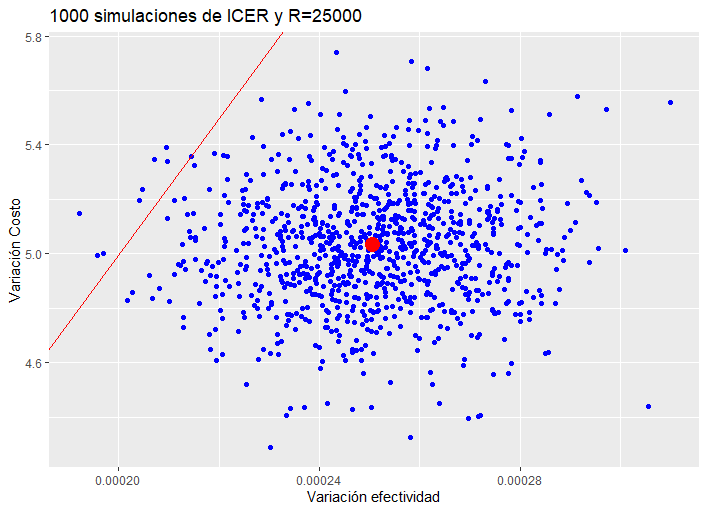
\includegraphics[width=0.45\textwidth]{grafi/mil_sims.png}
	\caption{Diferencia de efectividad y costos halladas en mil simulaciones} 
	\label{fig:3}   
\end{figure}

En este caso se supuso una distribución para la efectividad de la forma $\Delta_\epsilon \sim N(\bar{e_1}-\bar{e_0},\frac{\sigma_1^2}{n_1}+\frac{\sigma_0^2}{n_0})$ donde el sub-índice 1 indica que son los datos de vacunación y el sub-índice 0 para los datos sin vacunación, siguiendo el mismo procedimiento se siguió para la distribución de los costos.\\

Por último, se  puede hallar la curva de aceptación del nuevo tratamiento, con distintos valores de \textbf{R} se calcula la proporción de simulaciones que tienen \textbf{ICER} menor al valor de \textbf{R}, observando que a mayor valor de R, más proporción de ICER's simulados van a estar por debajo.\\

\begin{figure}[htbp]
	\centering
	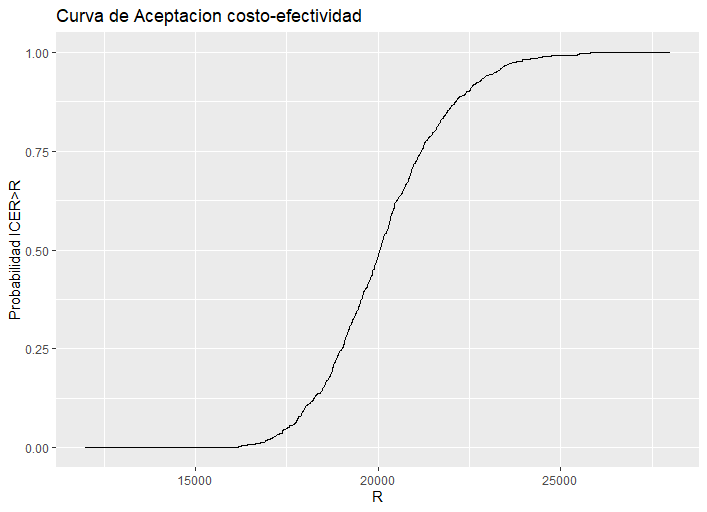
\includegraphics[width=0.4\textwidth]{grafi/curva_acept.png}
	\caption{Curva de Aceptación}
	\label{fig:4}
\end{figure}

\subsubsection{Aproximación mediante Bootstrap No Param\'etrico}
\label{sec:AMBNP}
Otra forma de resolver es mediante bootstrap no param\'etrico donde en general, se toma a la muestra cómo la población, y re-muestra nuevamente, repitiendo el proceso muchas veces de forma computacional, para poder estimar una estimación del parámetro de interés, la varianza e intervalos de confianza. En particular se utiliza el bootstrap para estimar la variación de la efectividad y la variación de los costos, y sus respectivos intervalos de confianza.Con estas estimaciones podremos graficar en el plano costo-efectividad tantos puntos cómo iteraciones hallamos hecho, representando estos puntos una pareja $(\Delta\epsilon,\Delta\gamma)$ de una iteración.


\cite{willan_statistical_2006} proponen que se hagan $B$ pasos, y en cada paso del bootstrap el tamaño de muestra de cada tratamiento sea igual a la cantidad de pacientes en cada tratamiento .Luego, para cada muestra se tendr\'a ($\hat{\Delta_{ei}},\hat{\Delta_{ci}}$), $\widehat{ICER_{i}}$, y fijado un R se podr\'a tener también $\widehat{INB_i}$ así cómo un estimador de la varianza y un intervalo de confianza.

\begin{figure}[htbp]
	\centering
	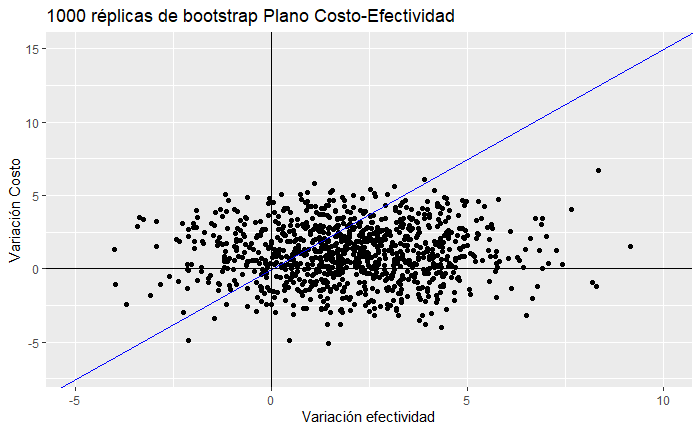
\includegraphics[width=0.45\textwidth]{grafi/boostrap.jpg}
	\caption{Representación de los ICER's para 1000 muestras obtenidas con bootstrap}
	\label{fig:5}
\end{figure}

El gráfico presentado en figura \ref{fig:5} no fue obtenido precisamente con el método de bootstrap, se hicieron mil simulaciones de dos normales, es meramente representativo.

\

Los intervalos de confianza basados en normalidad para el \textit{ICER} tienen serios problemas, ya que al ser un ratio, se vuelve muy inconsistente para valores de $\Delta_e$ muy cercanos a 0.

Se propone trabajar con intervalos de confianza construidos con el método de los percentiles, que además generan resultados consistentes para los tomadores de decisiones y replicables para el \textit{INB} y la curva de aceptación.


\subsection{Propuestas de  Planos de Efectividad con Frontera No Lineal}
\label{sec:PPEFNL}
En esta secci\'on se plantea una pequeña reflexión que surge luego de los planteos sobre el Plano Costo-Efectividad, el Ratio Incremental, y la disponibilidad a pagar.\\
En la simplificación de los problemas, cuando se compara la aplicación de un nuevo tratamiento vs el tratamiento actual, se ve que con el criterio aplicado con el ICER y el plano o con el INB se podía caer facilmente en la disminución de la efectividad del tratamiento, por el incremento del beneficio (en el bienestar social), si bien se comprende la definición del bienestar social, que implica estar dispuesto a la renuncia de la efectevidad por el implemento de un tratamiento más barato, por poder usar el dinero para otros fines, no pudimos dejar de lado que puede ser perjudicial que se pierda efectividad en los tratamientos, y al usar una frontera lineal, se veía que había iguales probabilidades de aumentar la efectividad que de disminuirla, por eso se plantean dos propuestas para la frontera de decisión del plano costo-efectividad que van en favor de los pacientes de interes para los tratamientos.\\

La primer propuesta, más sencilla, es que sea una función partida en función de $\Delta\epsilon$, con distintas pendientes para valores negativos y valores positivos. Se propone valores de $R$ y $R'$, tal que $R'>R$, entonces, para valores negativos de $\Delta\epsilon$ se tiene una pendiente mayor que valores positivos, entonces se exige mayor ahorro por cada unidad de efectividad perdida, que la disponibilidad a pagar a por una unidad extra de efectividad.

\begin{equation}
\Delta\gamma =
\begin{cases}
R  \text{  si  } \Delta\epsilon>0\\
R'  \text{  si  } \Delta\epsilon<0
\end{cases}
\end{equation}

\begin{figure}[htbp]
	\centering
	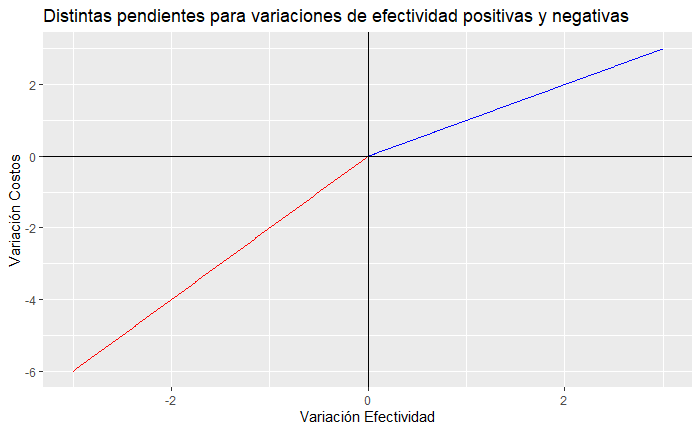
\includegraphics[width=0.45\textwidth]{grafi/Frontera_Partida.jpg}
	\caption{Representación de Plano Costo Efectividad con distintas pendientes de la frontera de aceptació}
	\label{fig:5}
\end{figure}


También presentaremos a continuación una frontera no lineal, que busca dar más probabilidad a aumentar, aunque sea un poco la efectividad, y para casos en los que se pierde efectividad, sigue el mismo razonamiento que la propuesta anterior. Lo negativo de este caso, es que el valor de R pierde poder de interpretación, aunque no cambie para valores positivos y negativos de la variación de efectividad.
Se nota, que si se toma límites de $\Delta\gamma-R*\Delta\epsilon$ tiende a 0 cuando $\Delta\epsilon$ tiende a infinito

\begin{equation}
\Delta\gamma =
\begin{cases}
R\Delta\epsilon \times(e^{-\Delta\epsilon} + 1)  \text{  si  } \Delta\epsilon>0\\
R\Delta\epsilon \times(e^{\Delta\epsilon} + 1)  \text{  si  } \Delta\epsilon<0
\end{cases}
\end{equation}

\begin{figure}[htbp]
	\centering
	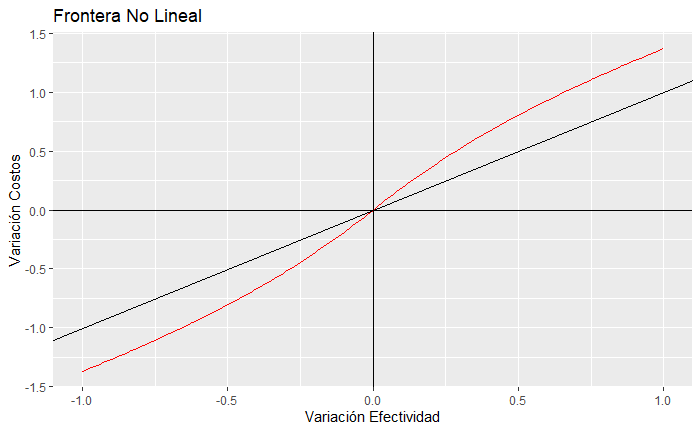
\includegraphics[width=0.45\textwidth]{grafi/Frontera_No_Lineal.jpg}
	\caption{Representación de Plano Costo Efectividad con Frontera No Lineal}
	\label{fig:6}
\end{figure}

\section{Conclusiones y futuros pasos}
\label{sec:Conclu}

En la secci\'on  \ref{sec:EE}  y en \ref{sec:EES} se presentan los problemas que dan origen a como  hacer la evaluaci\'on econ\'omica  y como en particular hacerlo en el \'ambito de de la saldu, doden surgen una serie de m\'etodos muy espec\'ificos que se han desarrollado para poder dar respuesta a  la forma de medir el costo que se asocia con dimensione muy  relevantes como son la Utilidad, el Beneficio y la Efectividad. Cada tipo de an\'alisis  tiene su m\'etricas asociadas y que corresponde tratarlas como variables aleatorias para la tomas de decisiones en condiciones de incertidumbre. El desarrollo elaborado en las secciones \ref{sec:AF} y \ref{sec:AMBNP} se basas en un enfoque frecuencista usando distribuciones de referencia  o aproximadas simuladas mediante bootstrap no param\'etrico. Por lo tanto  resta ver la ganancia que se logran al hacer un planteo desde una perspectiva bayesiana, y como futuros pasos se propone ver los resultados de usar simplificaciones en las m\'etricas  de An\'alisis de Costos con distribuciones conjugadas, compar\'andolos con los resultados de usar Cadenas de Markov Monte Carlo (MCMC). En particular las aplicaciones que se propone hacer son sobre el impacto de planes de vacunaci\'on para la gripe y para costo  en necesidades de pr\'otesis dentales  en poblaci\'on adulta en Uruguay.
%\begin{figure}[!b]
% \centering
%  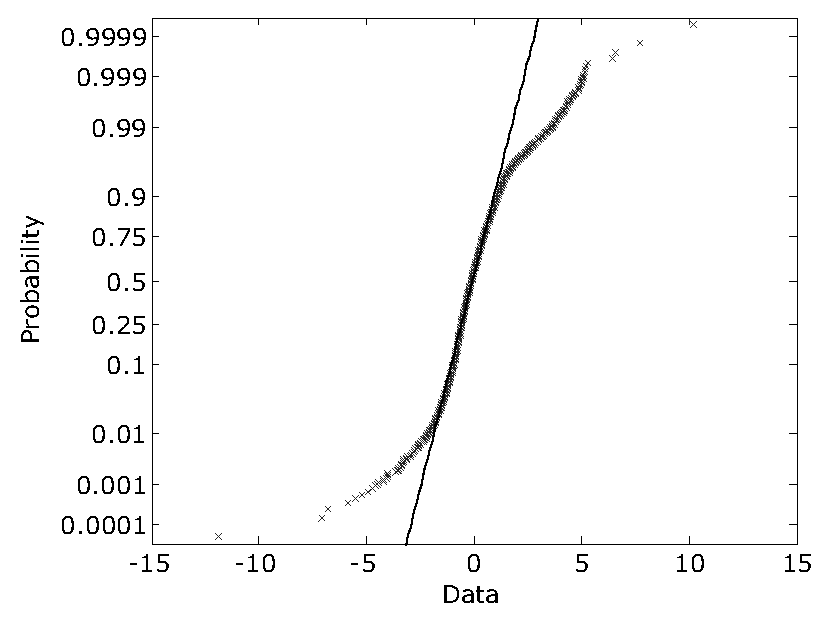
\includegraphics[width=0.45\textwidth]{fig1}
% \caption{Figure example.}
%  \label{fig1}
%\end{figure}









\bibliography{biblio/evaluacion_economica_salud.bib}

%\begin{thebibliography}{99}
%
%\bibitem{Bernard2} Bercu, Proia, {\em A sharp analysis on the asymptotic behavior of the Durbin-Watson statistic for the first order autoregresive process}, ESAIMPS, Vol. 16, 2012.
%
%\bibitem{tesisL} P\'erez Amaro, {\em Procesos auto-recursivos de orden uno, su relaci\'on con las martingalas y su aplicaci\'on en la predicci\'on de ciclones en M\'exico}, Tesis de Licenciatura, 2013.
%
%\end{thebibliography}

%\bibliography{amcs}




%\begin{appendix}{}
% The proof of Theorem 1 xx xxx xxx xxx xx xx xxx xxx xxx xxx xxxxx xx xx xxxx xx xx xxx xx xxx xxx xxx xx xx  xxx xxx xxx xxx xxxxx xx xx xxxx xx xx xxx.
%\begin{lemma}{}
%\end{lemma}
%\end{appendix}




%\makeinfo

\end{document}
